\documentclass[11pt,a4paper]{article}

% basic packages
\usepackage{float}
\usepackage{fullpage}
\usepackage{polski}
\usepackage{amsmath}
\usepackage{graphicx}
\usepackage[utf8x]{inputenc}

% arrow symbol
\usepackage{pifont}

% graphs
\usepackage{tikz}
\usetikzlibrary{arrows}

% bibliography and links
\usepackage{url}
\usepackage{cite}
\def\UrlBreaks{\do\/\do-}
\usepackage[hidelinks]{hyperref}

% listings 
\usepackage{listings}
\usepackage{color}
\definecolor{dkgreen}{rgb}{0,0.6,0}
\definecolor{gray}{rgb}{0.5,0.5,0.5}
\definecolor{mauve}{rgb}{0.58,0,0.82}
\lstset{
  basicstyle=\footnotesize,    
  captionpos=b,             
  commentstyle=\color{dkgreen},  
  frame=single,       
  keywordstyle=\color{blue},  
  language=Python,   
  numbers=left,     
  numbersep=7pt,   
  numberstyle=\tiny\color{gray}, 
  rulecolor=\color{black},  
  stringstyle=\color{mauve}, 
  tabsize=2,    
  title=\lstname
}

\begin{document}

\begin{titlepage}
  \begin{center}

    \textsc{\Large Politechnika Warszawska}\\[0.1cm]
    \small Wydział Elektroniki i Technik Informacyjnych
    \vfill

    \textsc{\small Współczesne techniki heurystyczne}\\[0.1cm]
    \Huge SK6. Algorytm przeszukiwania z~tabu dla problemu komiwojażera\\[1.5cm]
    \small Sprawozdanie 3\\[2.5cm]

    \vfill

    \begin{minipage}{0.4\textwidth}
      \begin{flushleft} \large
        \emph{Autorzy:}\\[0.1cm]
        Maciej \textsc{Suchecki}\\
        Jacek \textsc{Witkowski}\\
      \end{flushleft}
    \end{minipage}
    \begin{minipage}{0.4\textwidth}
      \begin{flushright} \large
        \emph{Prowadzący:}\\[0.1cm]
        dr~inż.~Sebastian \textsc{Kozłowski}\\[1cm]
      \end{flushright}
    \end{minipage}

    \vfill
    {\large \today}

  \end{center}
\end{titlepage}

\section{Część 1}
\subsection{Treść zadania}
\paragraph{Tytuł} SK6. Algorytm przeszukiwania z~tabu dla problemu komiwojażera
\paragraph{Opis} Należy zaimplementować algorytm przeszukiwania z tabu (wzbogacony w stosunku do wersji ,,klasycznej'' o elementy wskazane przez prowadzącego), a następnie zastosować ten algorytm do rozwiązania problemu komiwojażera.

\subsection{Implementacja}
\paragraph{Język programowania} Wybranym językiem programowania jest Java.
\paragraph{Założenia} Zakładamy, że badane grafy są niekierowane.
\paragraph{Reprezentacja rozwiązania} Rozwiązanie problemu będzie reprezentowane w postaci listy odwiedzanych miast (wierzchołków grafu).
\paragraph{Definicja sąsiedztwa} Generowanie sąsiadów zostanie zrealizowane na wzór algorytmu \textit{2-opt}~\cite{2opt}. Rozwiązaniem B sąsiednim do rozwiązania A nazywamy rozwiązanie powstałe po odwróceniu kolejności dowolnej części listy odwiedzonych miast.

\subsection{Element heurystyczny}
Algorytm przeszukiwania z~tabu~\cite{tabuSearch} jest nieefektywny w przypadkach, gdy ewaluacja sąsiednich rozwiązań jest czasochłonna. W takich przypadkach algorytm można usprawnić za pomocą metod heurystycznych. W tym wypadku chcemy zastosować metodę o nazwie ,,aspiration plus strategy''~\cite{aspirationPlus}.
\paragraph{Aspiration plus strategy} Strategia ta polega na heurystycznym wyborze sąsiada do dalszej ewaluacji. Do implementacji wybraliśmy strategię w wersji ze zmiennymi Min oraz Max. Zakłada ona ustalenie przed wykonaniem algorytmu trzech zmiennych: Plus, Min oraz Max. Oprócz tego należy ustalić próg aspiracji (threshold), który będzie minimum, przy którym algorytm powinien zaakceptować znalezione rozwiązanie. W~naszym wypadku będzie on generowany dynamicznie w~trakcie działania programu, na podstawie ewaluacji aktualnego najlepszego rozwiązania. Po ustaleniu ww. parametrów algorytm przeszukuje po kolei sąsiedztwo ostatniego rozwiązania, aż do znalezienia nowego rozwiązania z~jakością powyżej ustalonego progu. Następnie sprawdzane jest Plus kolejnych rozwiązań. Dodatkowo przyjętym usprawnieniem jest założenie, że liczba sprawdzonych rozwiązań nie będzie mniejsza od parametru Min oraz większa od parametru Max. Ze wszystkich sprawdzonych rozwiązań wybierane jest następnie rozwiązanie najlepsze.

\newpage
\section{Część 2}
\subsection{Główny algorytm programu}
\subsubsection{Pseudokod algorytmu przeszukiwania z Tabu}
\begin{lstlisting}[caption = Pseudokod algorytmu przeszukiwania z Tabu]
// glowny algorytm
findSolution(graph) {
  aspiration = generateAspirationLevel(graph);
  currentSolution = generateInitialSolution(graph);
  previousSolution = currentSolution;
  bestSolution = currentSolution;
  iterationsWithoutImprovement = 0;

  while (iterationsWithoutImprovement < 5) {
    neighbourhood = generateNeighbourhood(currentSolution);
    currentSolution = getBestNeighbour(neighbourhood, aspiration, bestSolution);

    addToTabuList(move(currentSolution));

    iterationsWithoutImprovement++;
    if (distance(currentSolution) < distance(previousSolution)) {
      iterationsWithoutImprovement = 0;
    }
    if (distance(currentSolution) < distance(bestSolution)) {
      bestSolution = currentSolution;
    }

    aspiration = adjustAspiration(aspiration, distance(bestSolution));
  }

  return bestSolution;
}
\end{lstlisting}

\subsubsection{Opis}
Algorytm na początku inicjalizuje zmienne początkowe (na podstawie badanego grafu, przekazanego w~zmiennej \textit{graph}). Następnie w~pętli generuje sąsiedztwo poprzednio wygenerowanego rozwiązania i za pomocą metody \textit{getBestNeighbour} wyszukuje najlepsze rozwiązanie z sąsiedztwa. Jeśli znalezione rozwiązanie jest lepsze od dotychczas najlepszego, zostaje zapisane. Ponadto -- ruch, który wygenerował z~poprzednio sprawdzanego rozwiązania aktualne najlepsze, zostaje zapisany na liście Tabu. Wszystkie opisane kroki są następnie powtarzane, dopóki w~pięciu kolejnych iteracjach nie uda nam się uzyskać poprawy rozwiązania. Dodatkowo, w~każdym kroku algorytmu poziom aspiracji jest korygowany.

\paragraph{Opis zmiennych}
\begin{itemize}
  \item \textit{aspiration} -- poziom aspiracji.
  \item \textit{currentSolution, previousSolution} -- aktualnie oraz poprzednio sprawdzane rozwiązanie.
  \item \textit{bestSolution} -- dotychczas najlepsze rozwiązanie.
  \item \textit{iterationsWithoutImprovement} -- liczba iteracji bez poprawy.
  \item \textit{neighbourhood} -- sąsiedztwo rozwiązania.
\end{itemize}

\paragraph{Opis funkcji}
\begin{itemize}
  \item \textit{generateAspirationLevel} -- generuje początkowy poziom aspiracji -- patrz sekcja~\ref{subsec:aspiracja}.
  \item \textit{generateInitialSolution} -- generuje początkowe rozwiązanie (listę wierzchołków grafu).
  \item \textit{generateNeighbourhood} -- generuje sąsiedztwo danego rozwiązania -- patrz sekcja~\ref{subsec:2opt}.
  \item \textit{getBestNeigbour} -- zwraca najlepszego sąsiada danego rozwiązania -- patrz sekcja~\ref{subsec:aspirationPlus}.
  \item \textit{adjustAspiration} -- zwraca nową wartość aspiracji -- patrz sekcja~\ref{subsec:aspiracja}.
  \item \textit{distance} -- zwraca długość ścieżki dla danego rozwiązania.
  \item \textit{move} -- zwraca ruch, który został wykonany do wygenerowania danego rozwiązania.
  \item \textit{addToTabuList} -- dodaje ruch do listy Tabu -- patrz sekcja~\ref{subsec:tabu}.
\end{itemize}

\subsection{Algorytm wyszukiwania najlepszego rozwiązania w sąsiedztwie}
\label{subsec:aspirationPlus}
\subsubsection{Pseudokod algorytmu wyszukiwania najlepszego rozwiązania w sąsiedztwie}
\begin{lstlisting}[caption = Pseudokod algorytmu wyszukiwania najlepszego rozwiązania w sąsiedztwie]
// wyszukiwanie najlepszego rozwiazania za pomoca Aspiration Plus Strategy
getBestNeighbour(neighbourhood, aspiration, bestSolution) {
  bestNeighbour = neighbourhood[0];
  neighboursChecked = 0;
  neighboursSinceAspirationSatisfied = 0;
  aspirationThresholdReached = false;

  for (every neighbour in neighbourhood) {
    if (moveShouldBeDone(neighbour, bestSolution, bestNeighbour)) {
      bestNeighbour = neighbour;
    }

    if(!aspirationThresholdReached) {
      aspirationThresholdReached = (distance(neighbour) < aspiration);
    }
    if (aspirationThresholdReached) {
      ++neighboursSinceAspirationSatisfied;
    }

    ++neighboursChecked;
    if (enoughSolutionsChecked()) break;
  }

  return bestNeighbour;
}

// sprawdzanie, czy powinno sie wykonac ruch
moveShouldBeDone(neighbour, bestSolution, bestNeighbour) {
  if (distance(neighbour) > distance(bestNeighbour) {
    return false;
  } else if (isTabu(move(neighbour))) {
    return distance(neighbour) < distance(bestSolution);
  }
  return true;
}
\end{lstlisting}

\subsubsection{Opis}
Algorytm wyszukuje najlepsze rozwiązanie z danego sąsiedztwa wykorzystując Aspiration Plus Strategy. Na początku odbywa się inicjalizacja zmiennych początkowych, opisanych poniżej. Następnie w pętli odbywa się sprawdzanie kolejnych rozwiązań, dopóki nie zostanie spełnione jedno z poniższych warunków:
\begin{enumerate}
  \item sprawdzono całe sąsiedztwo
  \item sprawdzono przynajmniej tyle rozwiązań, ile wynosi parametr \textit{max}
  \item ogólnie sprawdzono przynajmniej \textit{min} rozwiązań oraz od czasu spełnienia aspiracji sprawdzono przynajmniej \textit{plus} parametrów
\end{enumerate}

Powyższe warunki są sprawdzane przez funkcję \textit{enoughSolutionsChecked()}.\\

Ponadto, sprawdzany sąsiad jest przypisany do zmiennej \textit{bestNeighbour} tylko i wyłącznie wtedy, gdy jest lepszy od poprzedniego \textit{bestNeighbour} oraz spełnia warunek aspiracji lub nie znajduje się na liście Tabu.\\

Na końcu działania algorytmu zmienna \textit{bestNeighbour} jest zwracana jako reprezentująca najlepsze rozwiązanie.

\paragraph{Opis zmiennych}
\begin{itemize}
  \item \textit{neighbourhood} -- sąsiedztwo rozwiązania
  \item \textit{aspiration} -- poziom aspiracji
  \item \textit{bestNeighbour} -- dotychczas najlepszy sąsiad
  \item \textit{neighbour} -- aktualnie sprawdzany sąsiad
  \item \textit{neighboursChecked} -- liczba sprawdzonych jak dotąd sąsiadów
  \item \textit{neighboursSinceAspirationSatisfied} -- liczba sprawdzonych sąsiadów od kiedy poziom aspiracji jest spełniony
  \item \textit{aspirationThresholdReached} -- zmienna mówiąca, czy próg aspiracji został już osiągnięty.
\end{itemize}

\paragraph{Opis funkcji}
\begin{itemize}
  \item \textit{distance} -- zwraca długość ścieżki dla danego rozwiązania.
  \item \textit{move} -- zwraca ruch, który został wykonany do wygenerowania danego rozwiązania.
  \item \textit{isTabu} -- zwraca \textit{true}, jeśli ruch należy do listy Tabu -- patrz sekcja~\ref{subsec:tabu}.
  \item \textit{moveShouldBeDone} -- sprawdza, czy powinno się wykonać ruch do podanego sąsiada.
\end{itemize}

\newpage
\subsection{Generowanie sąsiedztwa}
\label{subsec:2opt}
\subsubsection{Opis}
Generowanie sąsiedztwa odbywa się za pomocą metody 2-opt. Metoda ta zakłada generowanie sąsiadów rozwiązania za pomocą odwrócenia kolejności miast w~dowolnej części ścieżki. Za pomocą dwóch indeksów oznacza się początek i~koniec odwracanego ciągu. Po wykonaniu takiej zamiany dla wszystkich możliwych indeksów \textit{i} oraz \textit{k}, otrzymujemy całe sąsiedztwo rozwiązania.

\subsubsection{Przykład}
W przykładzie wygenerujemy sąsiada ścieżki A \ding{213} B \ding{213} C \ding{213} D \ding{213} E \ding{213} F \ding{213} G \ding{213} H \ding{213} A, za~pomocą indeksów: i = 4, k = 7. Nowa ścieżka zostanie wygenerowana w~trzech krokach:
\begin{enumerate}
  \item (A \ding{213} B \ding{213} C) -- dodanie początkowego fragmentu w~kolejności
  \item A \ding{213} B \ding{213} C \ding{213} (G \ding{213} F \ding{213} E \ding{213} D) -- dodanie środkowego fragmentu w~odwrotnej kolejności
  \item A \ding{213} B \ding{213} C \ding{213} G \ding{213} F \ding{213} E \ding{213} D (\ding{213} H \ding{213} A) -- dodanie końcowego fragmentu w~kolejności
\end{enumerate}

\subsection{Ustalanie progu aspiracji}
\label{subsec:aspiracja}
\subsubsection{Opis}
Próg aspiracji jest na początku ustalany na podstawie właściwości grafu wejściowego, a następnie dynamicznie korygowany. Wartość początkowa ustawiana jest na średnią wagę krawędzi pomnożoną przez liczbę wierzchołków grafu (patrz przykład poniżej).\\
Dodatkowo, w~trakcie działania programu próg jest weryfikowany -- jeśli zostanie znaleziona droga, która ma długość mniejszą niż aktualny próg aspiracji, próg zostaje zaktualizowany. Jego nowa wartość wynosi średnią arytmetyczną ze starej wartości progu aspiracji oraz najkrótszej jak dotąd znalezionej ścieżki.

\subsubsection{Przykład}
Dla pełnego grafu zdefiniowanego poniżej:\\

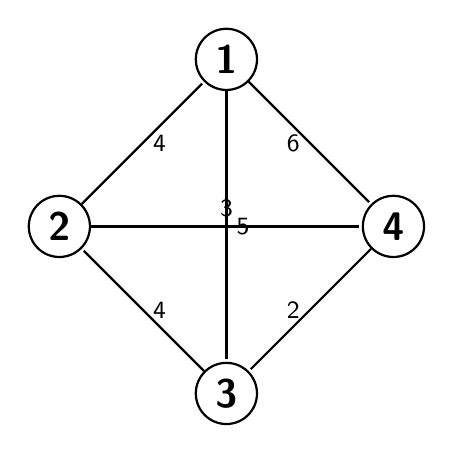
\begin{tikzpicture}[-,>=stealth',shorten >=1pt,auto,node distance=3cm,
  thick,main node/.style={circle,draw,font=\sffamily\Large\bfseries}]

  \node[main node] (1) {1};
  \node[main node] (2) [below left of=1] {2};
  \node[main node] (3) [below right of=2] {3};
  \node[main node] (4) [below right of=1] {4};

  \path[every node/.style={font=\sffamily\small}]
  (1) edge node [left] {6} (4)
  edge node {5} (3)
  (2) edge node [right] {4} (1)
  edge node {3} (4)
  (3) edge node [right] {4} (2)
  (4) edge node [left] {2} (3);
\end{tikzpicture}\\

\noindent Uzyskamy następującą początkową wartość poziomu aspiracji:\\
\begin{math}
  a = v * \frac{\sum w_e}{e} = 4 * \frac{4 + 6 + 3 + 5 + 4 + 2}{6} = 4 * \frac{24}{6} = 16
\end{math}

\subsection{Obsługa listy Tabu}
\label{subsec:tabu}
\subsubsection{Opis}
\textit{TabuList} jest kontenerem przechowującym listę ruchów zabronionych do wykonania w poszukiwaniu lepszych rozwiązań. Ruch określony jest poprzez dwa punkty podziału rozwiązania (generowanego metodą 2-opt).\\

Kontener zapewnia szybkie sprawdzanie (w czasie stałym), czy dany ruch jest zabroniony (tj. znajduje się w~kontenerze), jak również szybkie dodawanie nowego ruchu (również w czasie stałym). Dodatkowo kontener ,,pamięta'' kolejność dodawania ruchów do listy tabu. Dzięki temu w przypadku przekroczenia maksymalnej liczby ruchów przechowywanych w kontenerze, możliwe jest usunięcie najdawniej dodanego ruchu do kontenera (operacja wykonywana automatycznie).\\

By zapewnić szybkie sprawdzanie czy ruch znajduje się w kontenerze wykorzystano kontener \textit{HashMap}. By pamiętać kolejność dodawanych ruchów wykorzystano listę typu \textit{LinkedList}.

\newpage
\section{Część 3}
\subsection{Prezentacja wyników}
\subsubsection{Definicje}
W~kontekście testowania projektu definiujemy dwa parametry określające wydajność algorytmu:
\begin{itemize}
  \item \textbf{wynik} -- długość najkrótszej ścieżki znalezionej przez program (jakość rozwiązania),
  \item \textbf{czas działania programu} -- czas, jaki upłynął pomiędzy wykonaniem programu (dla zadanych parametrów oraz grafu wejściowego), a jego zakończeniem i~zwróceniem wyniku.
\end{itemize}

\subsubsection{Uśrednianie wyników}
Ze względu na fakt, iż zaimplementowany algorytm jest algorytmem heurystycznym, jakość otrzymywanych wyników zależy od właściwości grafu podanego na wejściu. Z~tego powodu -- dla zwiększenia czytelności wyników -- każde uruchomienie programu jest powtarzane kilkukrotnie dla różnych grafów. Wynik oraz czas działania programu jest przyjmowany jako średnia z~odpowiednich wartości w~kolejnych uruchomieniach.\\

Liczba powtórzeń była wyznaczona doświadczalnie, za pomocą eksperymentu przedstawionego na wykresie poniżej:
\begin{figure}[H]
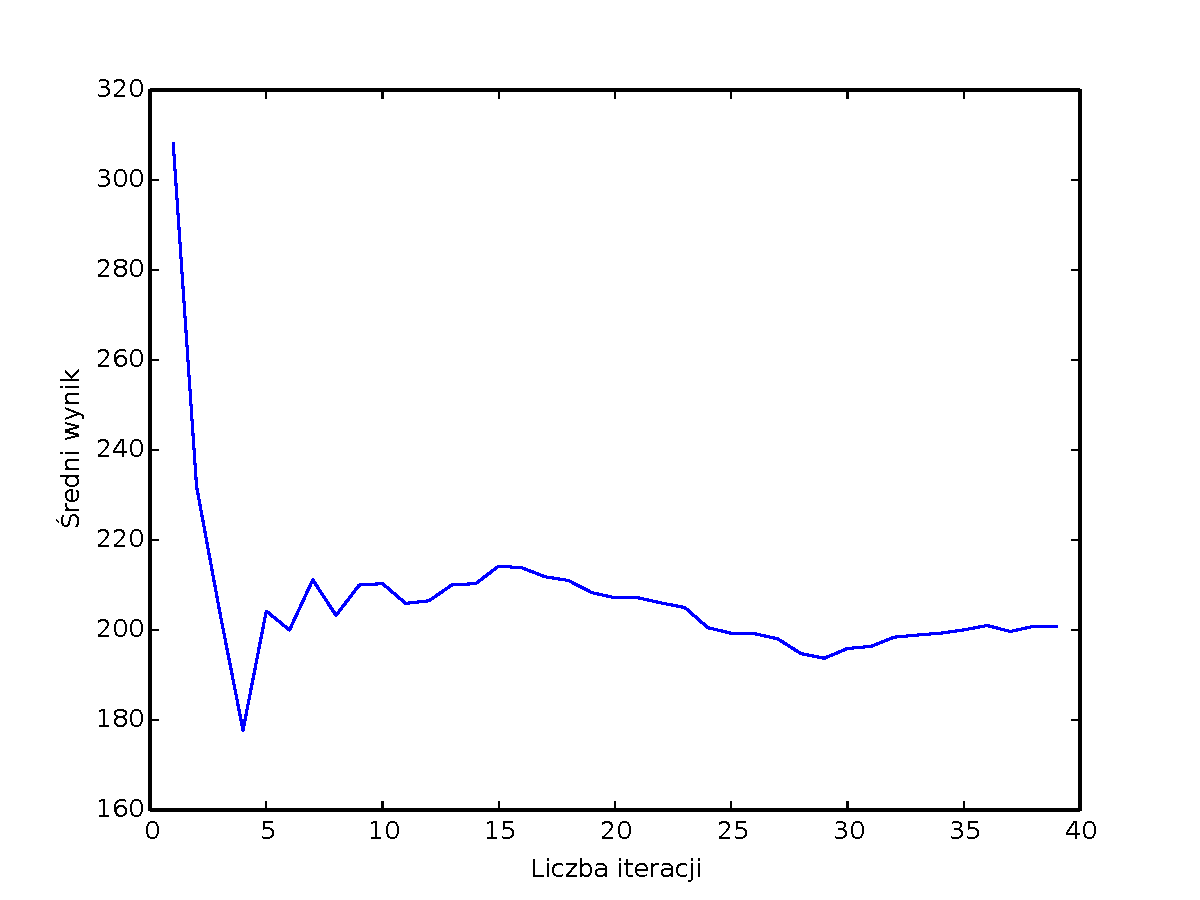
\includegraphics[trim = 0mm 0mm 0mm 12mm, clip, width=14cm]{graphs/repetitions.pdf}
\caption{Zależność średniego wyniku działania programu od liczby powtórzeń}
\end{figure}

W~celu wyznaczenia liczby powtórzeń, wygenerowaliśmy 50 losowych grafów pełnych. Następnie uruchamialiśmy solver dla coraz większej liczby grafów, uśredniając przy tym otrzymany wynik. Na otrzymanym wykresie widać, że wartość 10 jest minimalną liczbą powtórzeń, dla których można już potwierdzić wiarygodność otrzymywanych wyników.\\

\newpage
Kod generujący powyższy wykres jest przedstawiony poniżej:

\begin{lstlisting}[caption = Fragment kodu programu w języku Python generującego powyższy wykres]
# parameters
maxIterations = 50
graphSize =  10

# generate graphs
filenames = graph.saveRandomGraphsToFiles(maxIterations, graphSize)

# collect data
averageResults = {}
for iterations in range(1, maxIterations):
  averageResult = 0
  for i in range(iterations):
    averageResult += runSolver(filenames[i])
  averageResults[iterations] = averageResult / iterations

plotGraph(averageResults, "Liczba iteracji", "Sredni wynik")
\end{lstlisting}

\subsubsection{Badanie wpływu parametrów na wydajność algorytmu}
Po wyznaczeniu wymaganej liczby powtórzeń został utworzony skrypt testujący. Generuje on na początku 10 losowych grafów. Następnie uruchamia solver dla poszczególnych kombinacji parametrów. Uzyskane wyniki wraz z~czasami wykonania programu są zapisywane w~celu wykonania na ich podstawie wykresów, które zaprezentowane są poniżej.

\subsubsection{Wpływ rozmiaru listy Tabu na wydajność algorytmu}
\begin{figure}[H]
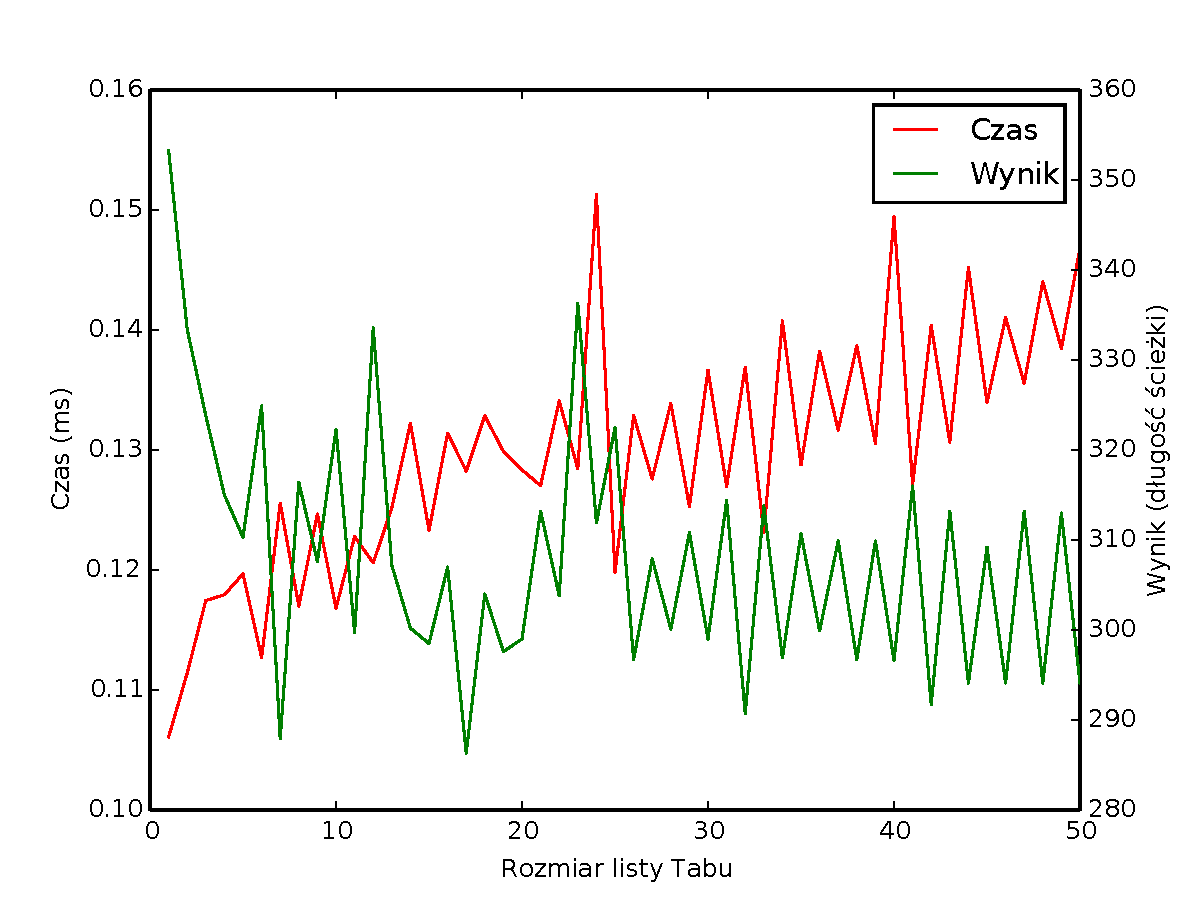
\includegraphics[trim = 0mm 3mm 0mm 12mm, clip, width=14cm]{graphs/tabuListSize.pdf}
\caption{Wpływ rozmiaru listy Tabu na wydajność algorytmu.}
\end{figure}

\subsubsection{Wpływ parametru Plus na wydajność algorytmu}
\begin{figure}[H]
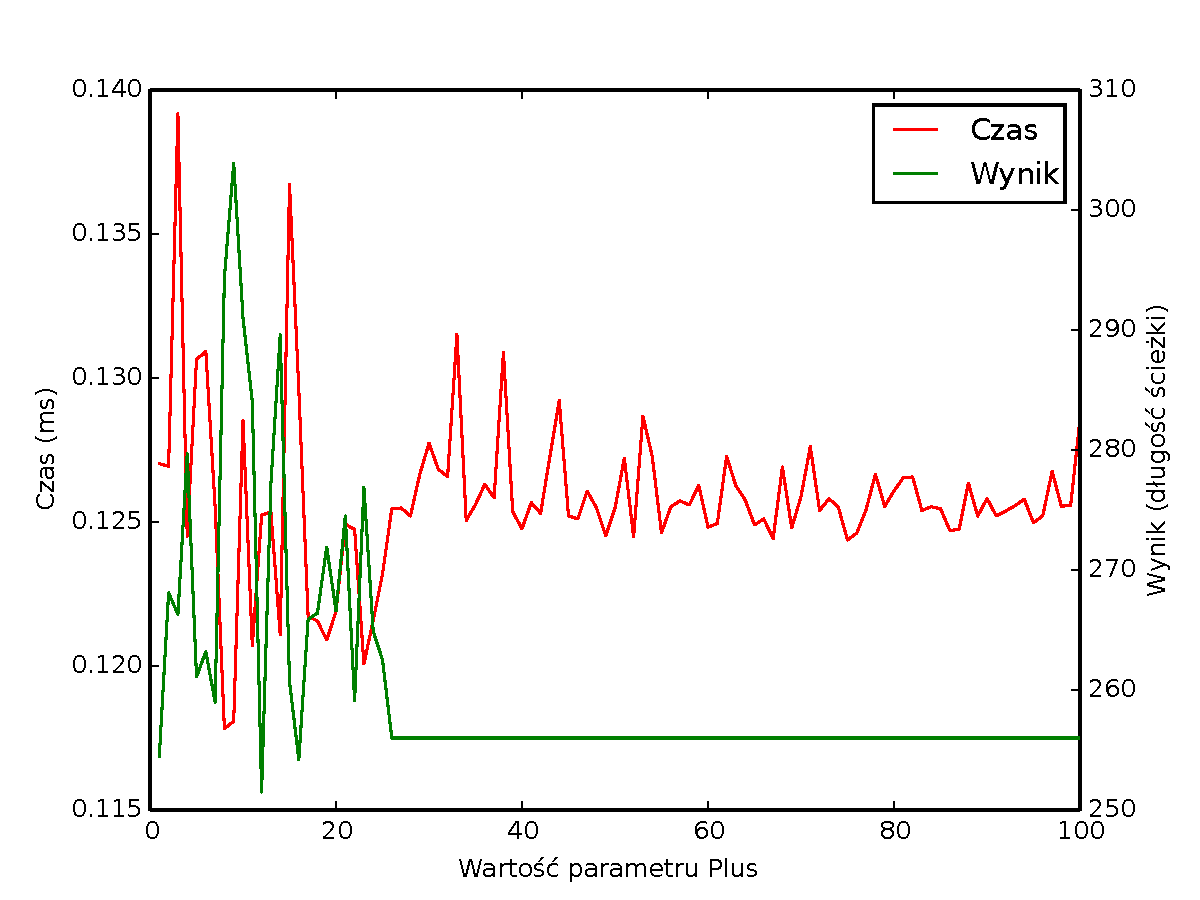
\includegraphics[trim = 0mm 3mm 0mm 12mm, clip, width=14cm]{graphs/plus.pdf}
\caption{Wpływ parametru Plus na wydajność algorytmu.}
\end{figure}

\subsubsection{Wpływ parametru Min na wydajność algorytmu}
\begin{figure}[H]
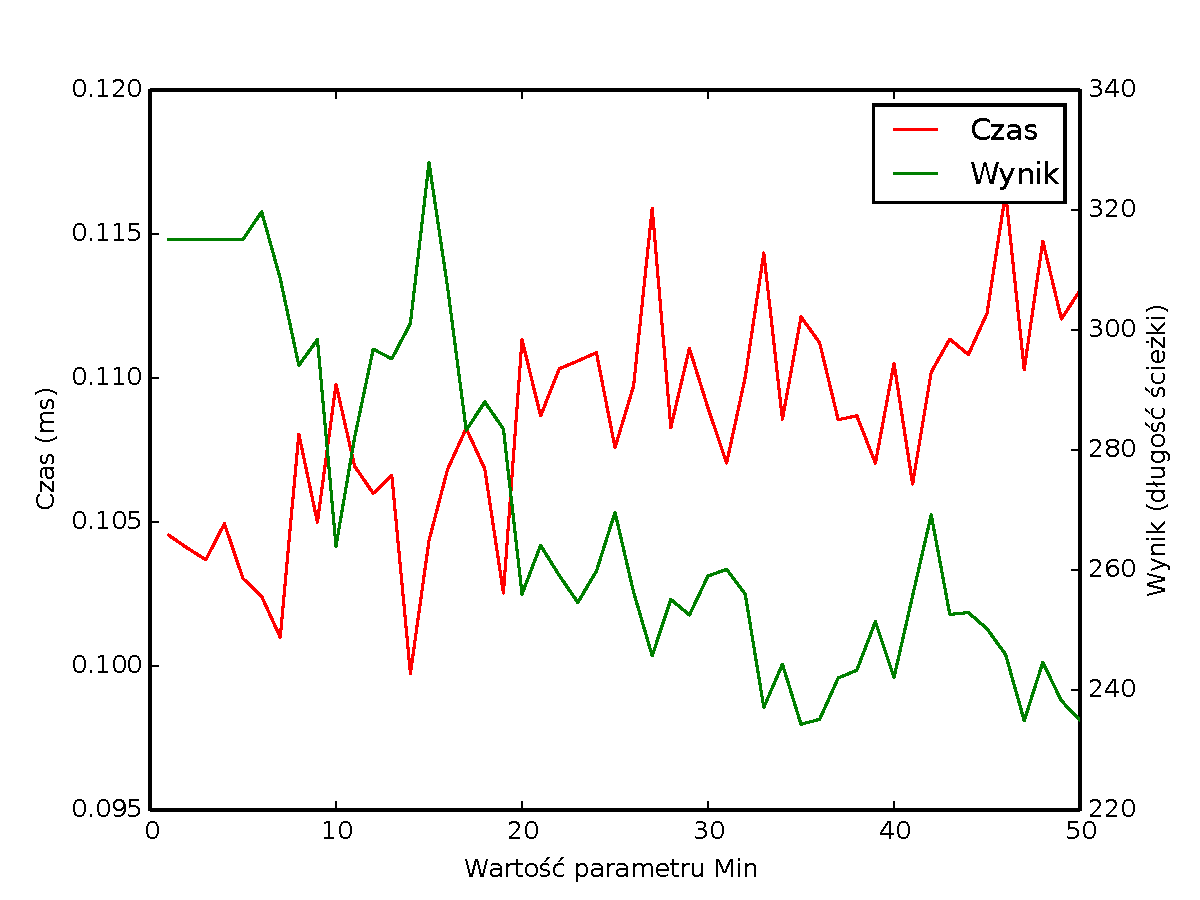
\includegraphics[trim = 0mm 3mm 0mm 12mm, clip, width=14cm]{graphs/min.pdf}
\caption{Wpływ parametru Min na wydajność algorytmu.}
\end{figure}

\newpage
\subsubsection{Wpływ parametru Max na wydajność algorytmu}
\begin{figure}[H]
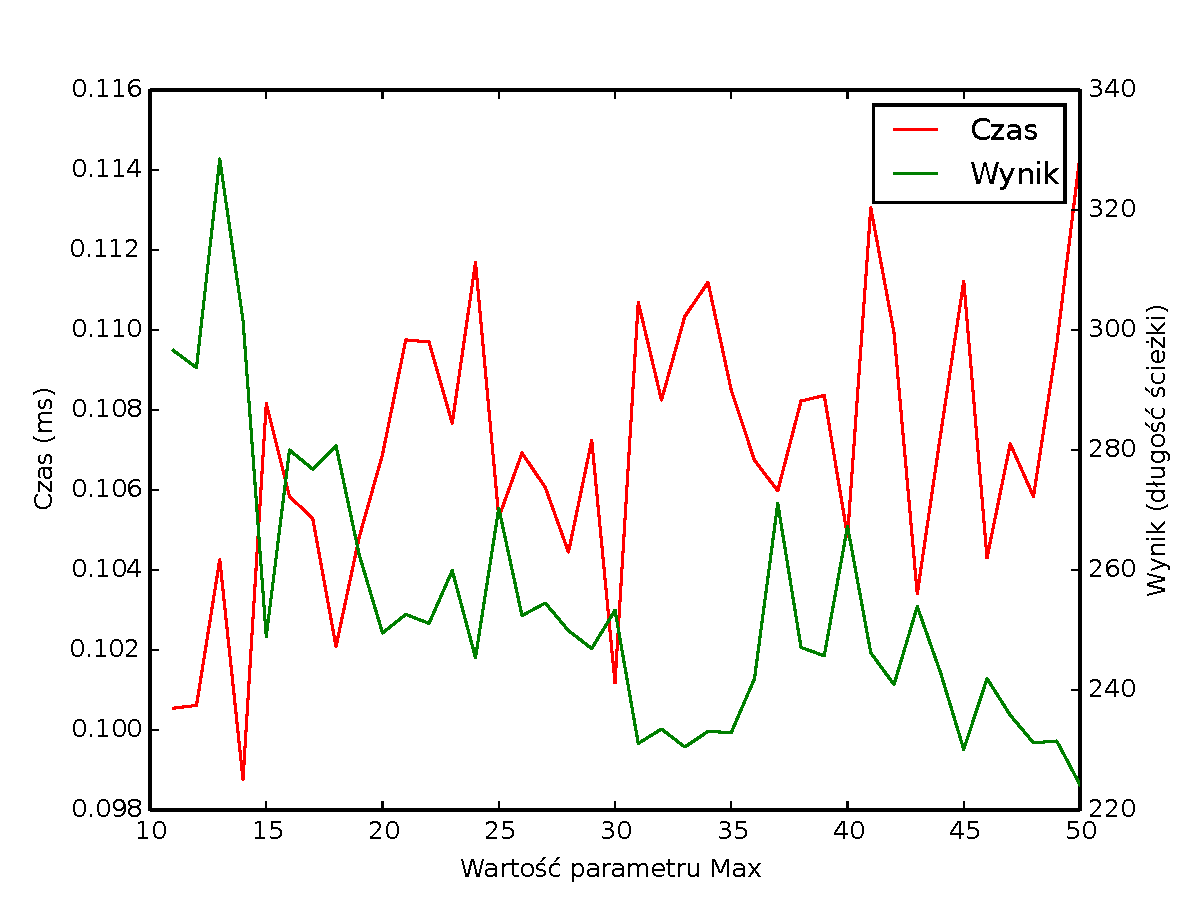
\includegraphics[trim = 0mm 3mm 0mm 12mm, clip, width=14cm]{graphs/max.pdf}
\caption{Wpływ parametru Max na wydajność algorytmu.}
\end{figure}

\subsubsection{Wnioski}
Uzyskane wyniki są zgodne z~naszymi oczekiwaniami. Po pierwsze, dla wszystkich parametrów widać wyraźny wpływ na czas działania algorytmu -- zwiększanie wartości każdego z~parametrów powoduje zasadniczo zwiększenie czasu wykonywania algorytmu. Jest to zgodne z~intuicją, ponieważ zwiększenie każdego z~parametrów powoduje zwiększenie liczby rozwiązań koniecznych do sprawdzenia, a~co za tym idzie -- liczby operacji do wykonania.\\

Z~tego samego powodu na wykresach można wyraźnie zaobserwować polepszanie się znalezionego rozwiązania wraz ze zwiększaniem parametrów. Ciekawe są zwłaszcza pierwsze dwa wykresy. W~przypadku listy Tabu, można zaobserwować oscylacje na końcu wykresu. Odnośnie parametru Plus, widać ustabilizowanie się wyniku dla wartości powyżej 25 -- zwiększanie parametru nie daje poprawy ze względu na ograniczony rozmiar sąsiedztwa rozwiązania. \\

Na podstawie dokładniejszej analizy wykresów można wyznaczyć optymalne wartości parametrów dla tak zaimplementowanego algorytmu. Oczywiście zależą one od konkretnego grafu (w~szczególności oczywiście od liczby wierzchołków) oraz naszych priorytetów (szybkość/jakość) aczkolwiek w~ogólności prezentują się one według nas następująco:
\begin{itemize}
  \item rozmiar listy Tabu: optymalna wartość zawiera się w~przedziale (15, 25)
  \item parametr Plus: optymalna wartość zawiera się w~przedziale (25, 35)
  \item parametr Min: optymalna wartość zawiera się w~przedziale (20, 50)
  \item parametr Max: optymalna wartość zawiera się w~przedziale (20, 50)
\end{itemize}

% bibliography
\addcontentsline{toc}{chapter}{Bibliografia}
\bibliography{references}{}
\bibliographystyle{alpha}

\end{document}
